
\documentclass[11pt, a4paper]{article}
%\usepackage{proj1}
\usepackage{natbib}
\usepackage{fancyhdr}  
\usepackage{subcaption}
\usepackage{caption}
\usepackage{graphicx}
\usepackage{numprint}
\usepackage{multirow}
\linespread{1.25} 
\setlength{\parindent}{0cm}
\graphicspath{{Images/}}
\usepackage{hyperref}
\usepackage{amsmath}
\usepackage{amsfonts}
\usepackage{amssymb}
\usepackage{amsthm}
\usepackage{mathtools}
\usepackage{commath}
\usepackage{bbm}

%\usepackage[sc,osf]{mathpazo}
\usepackage{subcaption}
\usepackage[a4paper, top=1in, left=1.0in, right=1.0in, bottom=1in, includehead, includefoot]{geometry} %Usually have top as 1in

\usepackage{listings}
\usepackage{color} %red, green, blue, yellow, cyan, magenta, black, white
\definecolor{mygreen}{RGB}{28,172,0} % color values Red, Green, Blue
\definecolor{mylilas}{RGB}{170,55,241}


\hypersetup{colorlinks,linkcolor={black},citecolor={blue},urlcolor={black}}
\usepackage{color}
\urlstyle{same}


\theoremstyle{definition}
\newtheorem{definition}{Definition}[section]

\newcommand{\adja}{q_a}
\newcommand{\adjb}{q_b}
\newcommand{\adjaB}{q_{a,\partial \Omega}}
\newcommand{\adjbB}{q_{b,\partial \Omega}}
\newcommand{\adjB}{q_{\partial \Omega}}
\newcommand{\Adja}{\mathbf{p}}
\newcommand{\Adjb}{q}
\newcommand{\adj}{q}
\newcommand{\Adjc}{{q}_{\partial \Omega}}
\newcommand{\ra}{\rho_a}
\newcommand{\rb}{\rho_b}
\newcommand{\w}{\mathbf{w}}
\newcommand{\f}{\mathbf{f}}
\newcommand{\ve}{\mathbf{v}}
\newcommand{\n}{\mathbf{n}}
\newcommand{\h}{\mathbf{h}}
\newcommand{\K}{\mathbf{K}}
\newcommand{\hr}{\widehat \rho}
\newcommand{\jf}{\mathbf j}

\DeclareMathOperator{\sgn}{sgn}
\DeclareMathOperator{\Grad}{Grad}
\DeclareMathOperator{\Div}{Div}
\DeclareMathOperator{\Lap}{Lap}
%	\begin{figure}[h]
%		\centering
%		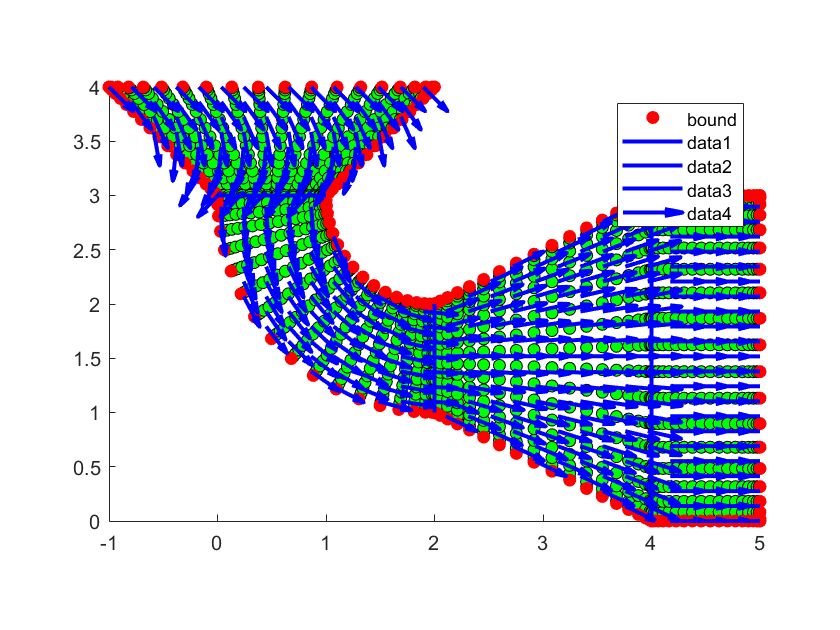
\includegraphics[scale=0.35]{F1.png}
%		\caption{Forward $\rho$ for $a = 0.01$} 
%		\label{F1}
%	\end{figure}

\begin{document}
	\section*{D 21/04/2021}
Notes	
	\begin{itemize}
		\item Interpolation works now (also for periodic functions)
		\item Shape notes/ multishape tests complete, except for questions and convergence stuff
		\item Tested the 'VectorToShape' for w and when to use
		\item DDFT talk (maybe different example?)
		\item ALOP Workshop
	\end{itemize}
Questions
	\begin{itemize}
		\item Reference for exact no-flux AD solution?
		\item Plotting single normals
		\item Polar Diff at $r=0$?
		\item Wedge linear, quadrilateral bilinear. why?
		\item Algorithm writing (how to improve this)
		\item Loewen paper: $N = 100$ -  how to translate to $\rho$
		\item Loewen $V_{ext}$ problem: Do we do $V_2$ as well? Interesting $\hr$? 
		\item $\nabla V_{ext}$ control 'constant' -  spatial averaging?
		\item Is DDFT valid for $\w$ which is not $\nabla V$? (see DDFT review 3.4/4.4 - need diffusion dominated flow?)
	\end{itemize}
	\section{Separation Example}
	We model a separation example with the external potential
	\begin{align*}
		V_{ext} = 10 \left(\frac{r}{4 \sigma}\right)^4 + \cos(2 \pi t / 2.75) \left(\frac{r}{\sigma}\right)^2.
	\end{align*}
	We choose $\rho_0 = \bar \rho e^{-V_{ext}}$ and $\bar \rho = 0.05$. The domain is $[0,5]^2$ with $N = 30$ and $n = 60$. The time horizon is $(0,3)$. If we define $r = |y_1|$, the solutions for $\kappa = 1$ and $\kappa = -1$ for the sedimentation equation with corresponding $V_2$ are displayed in Figures \ref{F1} and \ref{F1a}. The results for the standard overdamped equation look very similar. The external potential is shown in Figure \ref{F1b}. The two-dimensional problem (meaning $r = \sqrt{y_1^2 + y_2^2}$) are essentially the same.
	\begin{figure}[h]
		\centering
		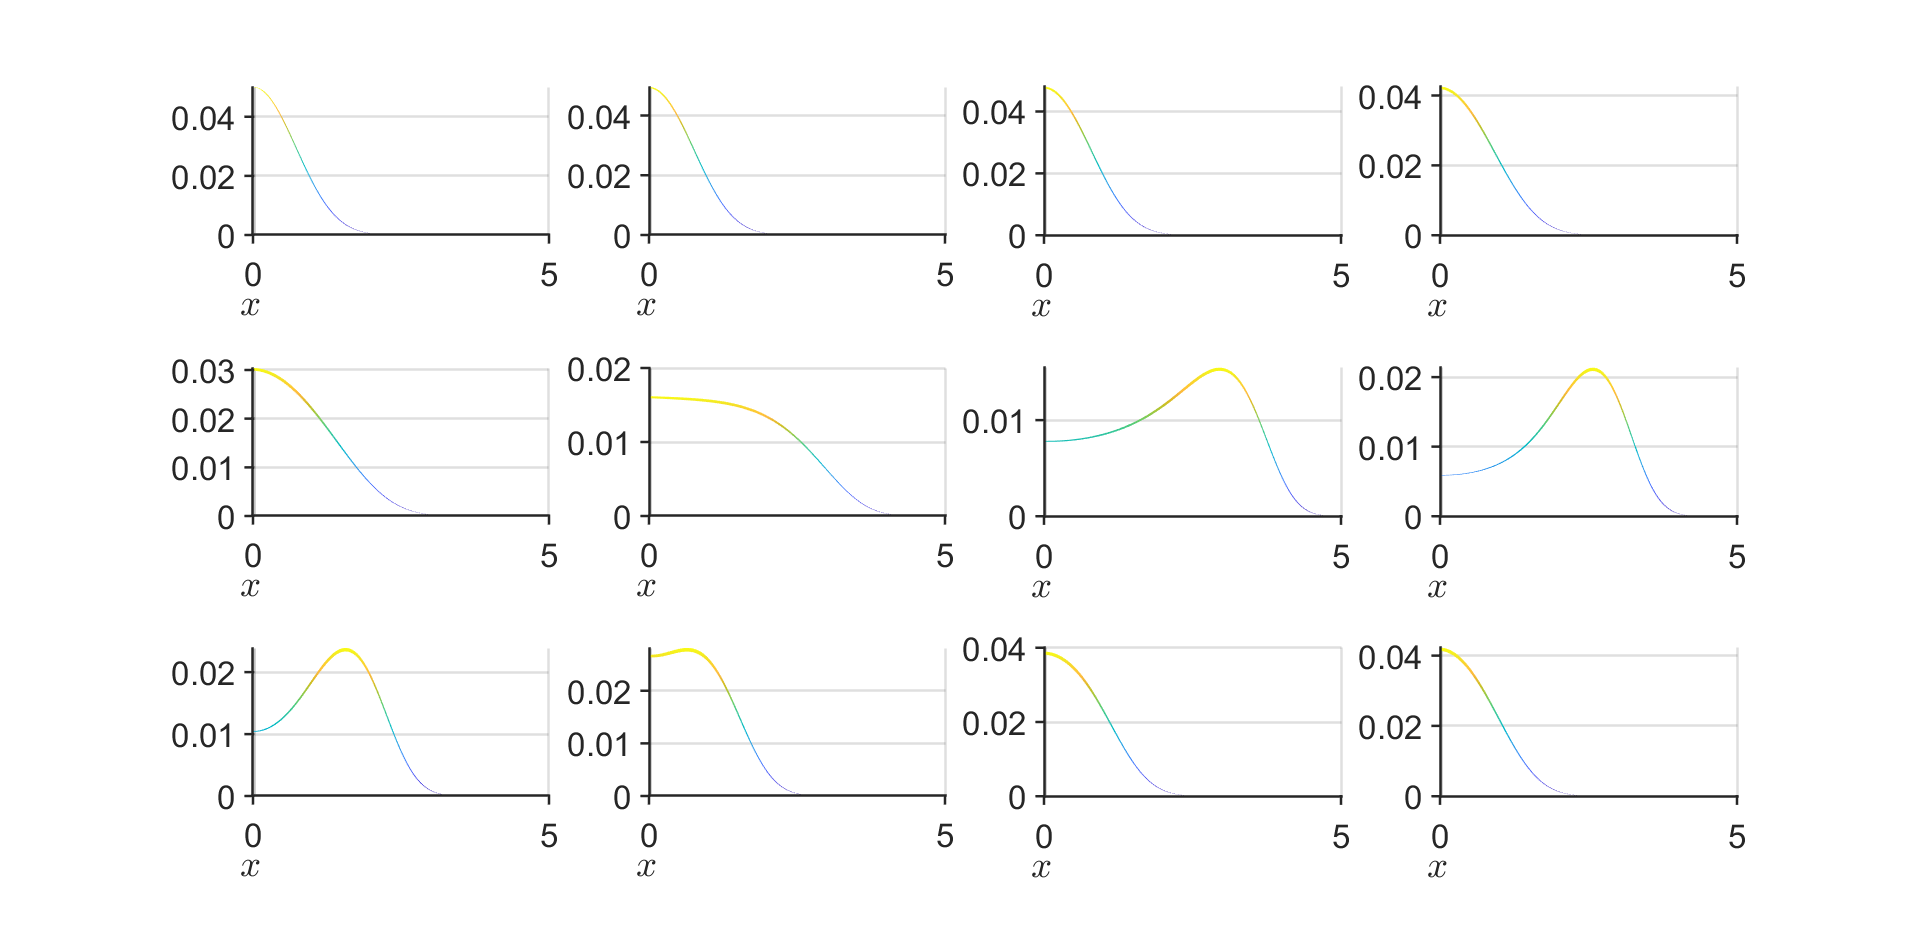
\includegraphics[scale=0.35]{Exkappa1.png}
		\caption{'1D' solutions for sedimentation, $\kappa = 1$} 
		\label{F1}
	\end{figure}
	\begin{figure}[h]
		\centering
		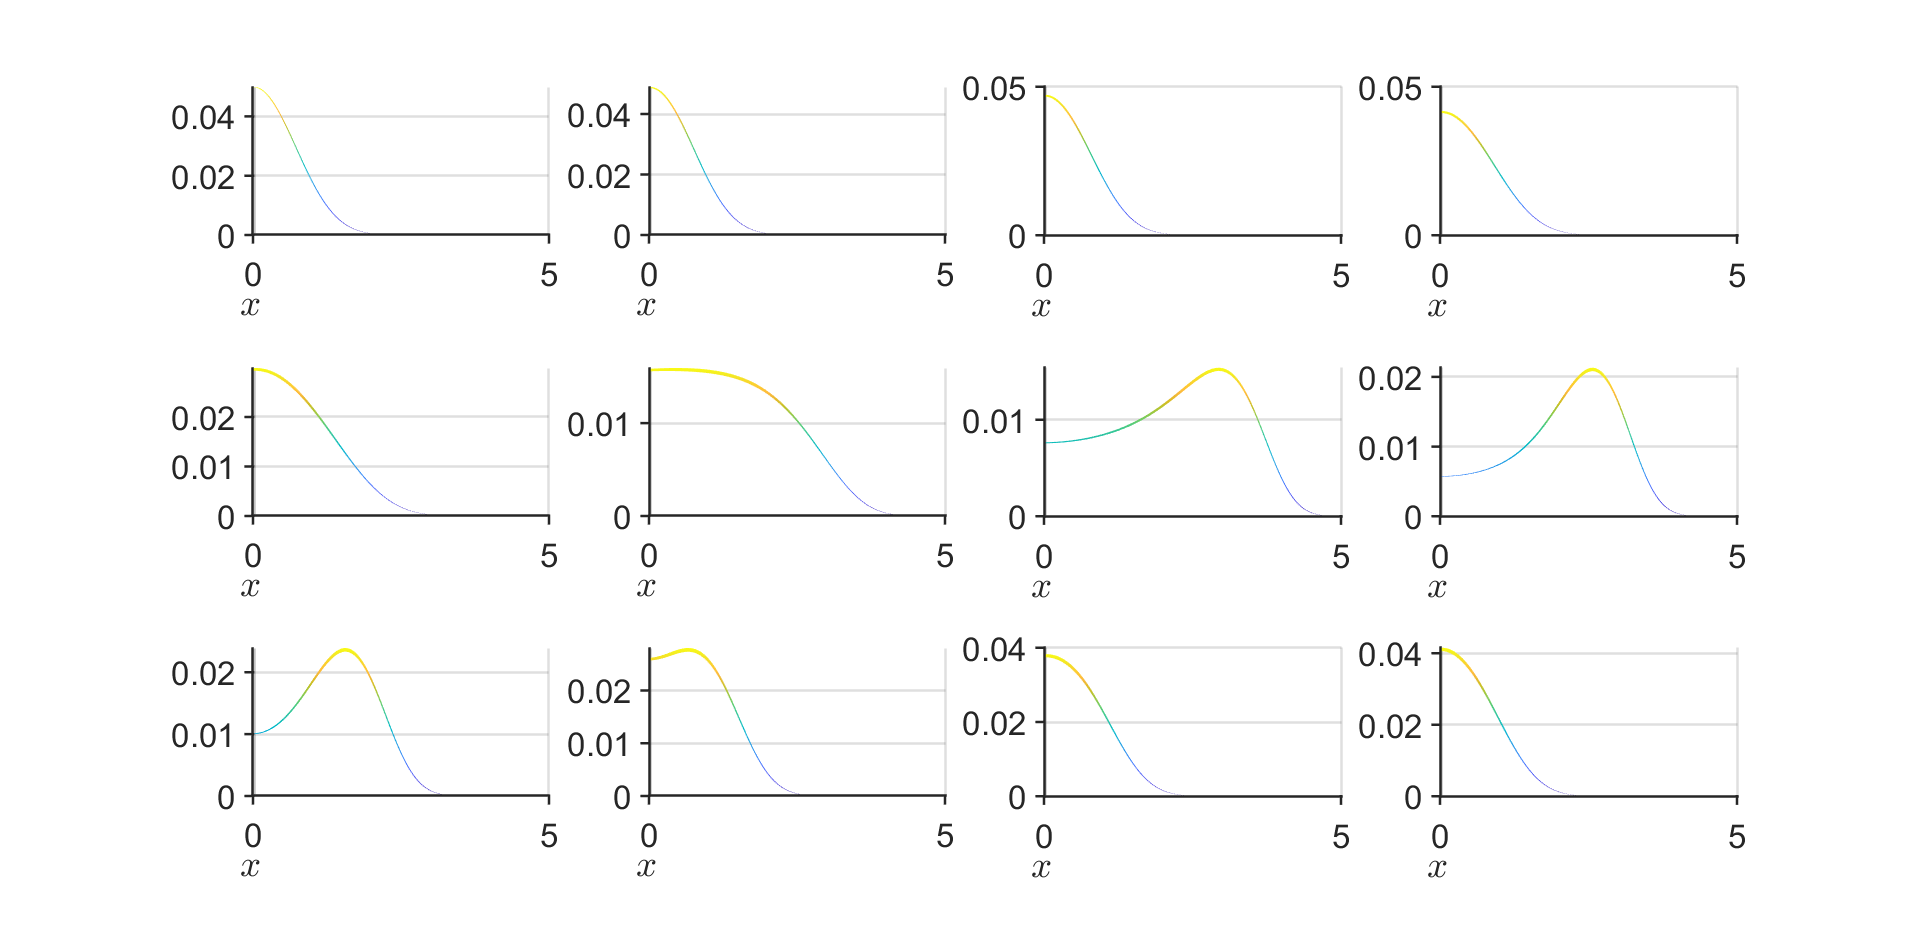
\includegraphics[scale=0.35]{Exkappan1.png}
		\caption{'1D' solutions for sedimentation, $\kappa = - 1$} 
		\label{F1a}
	\end{figure}
	\begin{figure}[h]
		\centering
		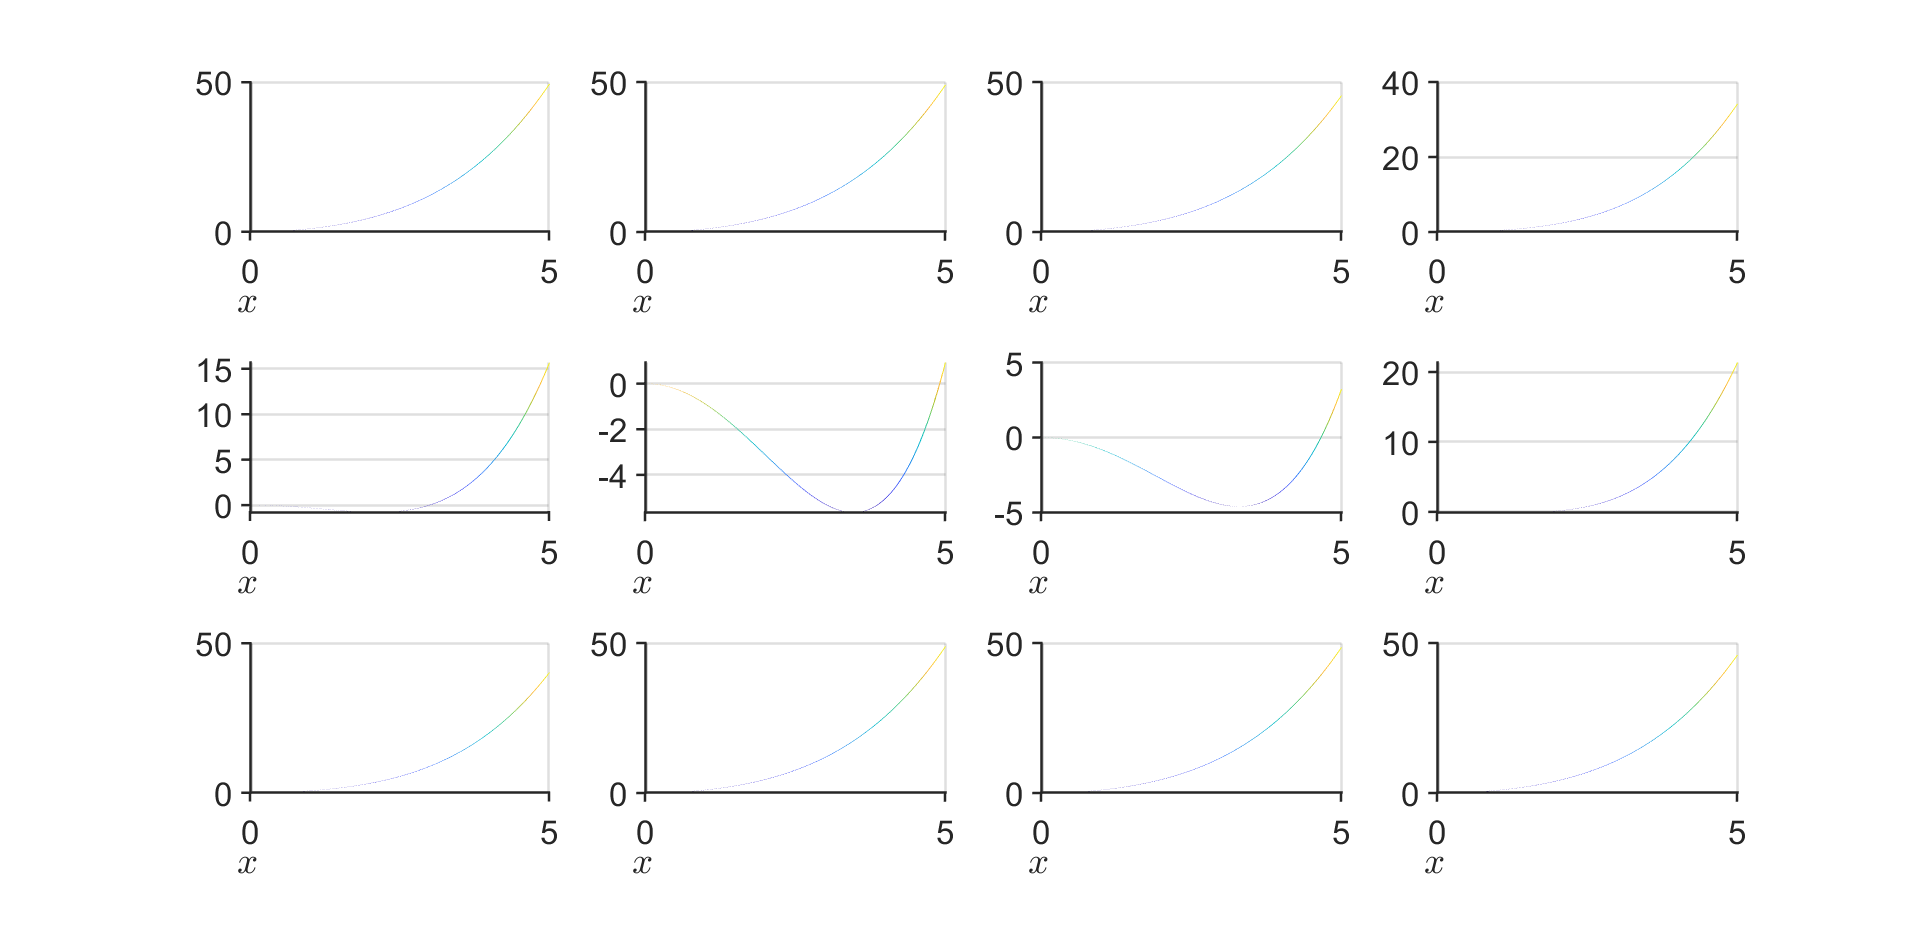
\includegraphics[scale=0.35]{Vext.png}
		\caption{'1D' $V_{ext}$} 
		\label{F1b}
	\end{figure}
	
\end{document}